\section{Leis de Kirchhoff}

As leis de Kirchhoff são utilizadas para analisar circuitos de forma a poder obter valores de parâmetros elétricos em pontos ou componentes específicos de um circuito.

A \textbf{primeira lei de Kirchhoff} fala sobre as correntes em um nó, por isso é comum ser chamada de \textbf{lei dos nós}, enquanto que a \textbf{segunda lei de Kirchhoff} fala sobre as tensões em uma malha, sendo assim a \textbf{lei das malhas}.





\subsection{Lei dos Nós - 1ª Lei de Kirchhoff}

A Figura \ref{fig:nosAeB} mostra o \textbf{sentido convencional} da corrente que flui do polo positivo para o polo negativo da fonte.
Entre o polo positivo da fonte e o nó $A$, tem-se a corrente total do circuito, $I_T$, que se divide nos dois ramos ali conectados em $I_1$ e $I_2$. Assim, a soma das correntes que saem do nó é igual a corrente que chega nele.
\begin{equation}
I_T = I_1 + I_2
\end{equation}

Da mesma forma no nó $B$, temos:
\begin{equation}
I_1 + I_2	= I_T
\end{equation}

\begin{figure}[!h]
	\centering
	\caption{Circuito em paralelo}
	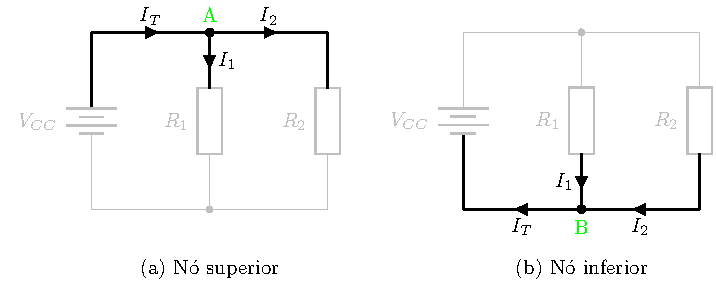
\includegraphics[scale=1.0]{fig-noSupInf}
	\label{fig:nosAeB}
\end{figure}

Pela definição da lei dos nós,
\textbf{A soma das correntes em um nó é igual a zero.}

Tendo um nó como referência, adota-se uma convenção para o sentido da corrente. Assim, a corrente que chega ao nó é anotada como positiva e a corrente que sai é negativa. O oposto também pode ser adotado.

Escrevendo, pela definição, a equação para o nó $A$ temos:
\begin{eqnarray}
\label{eq:1kirchhoff}
(+I_T) + (-I_1) + (-I_2) & = & 0\\
I_T - I_1 - I_2 & = & 0 \nonumber\\
I_T - I_1 - I_2 \color{blue}{+ I_1 + I_2}& = & 0 \color{blue}{+I_1 + I_2} \nonumber\\
I_T \cancel{-I_1} \cancel{- I_2} \color{blue}{\cancel{+ I_1} \cancel{+ I_2}}& = & \color{blue}{+I_1 + I_2} \nonumber\\
I_T & = & I_1 + I_2
\end{eqnarray}
Da mesma forma para o nó $B$:
\begin{eqnarray}
(-I_T) + (+I_1) + (+I_2) & = & 0 \nonumber\\
-I_T + I_1 + I_2 \color{blue}{+I_T}& = & 0\color{blue}{+I_T} \nonumber\\
\cancel{-I_T} + I_1 + I_2 \color{blue}{\cancel{+I_T}}& = & 0\color{blue}{+I_T} \nonumber\\
I_1 + I_2 & = & I_T \nonumber
\end{eqnarray}











\subsection{Lei das Malhas - 2ª Lei de Kirchhoff}

A Figura \ref{fig:malha} mostra os dois ramos que formam o circuito em série.
A limitação dos ramos são os nós $A$ e $B$, cuja diferença de potencial $V_{AB}$ é proporcionada pelo ramo da fonte, $V_{CC}$.
\begin{equation}
	V_{AB} = V_{CC}
\end{equation}
Essa diferença de potencial, é aplicada ao ramo que contém os resistores, $R_1$ e $R_2$, que dividem essa tensão em valores parciais, denominados de queda de tensão, $V_{R1}$ e $V_{R2}$. Então:
\begin{equation}
	V_{AB} = V_{R1} + V_{R2}
\end{equation}
\begin{figure}[!h]
	\centering
	\caption{Circuito em Série}
	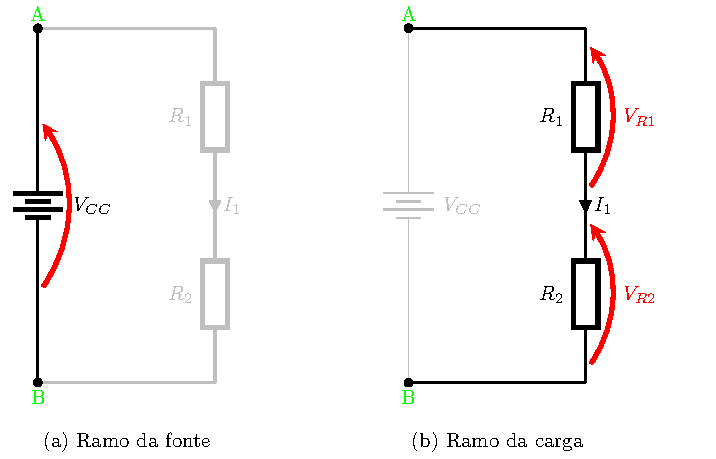
\includegraphics[scale=1.0]{fig-malha}
	\label{fig:malha}
\end{figure}

A segunda lei de Kirchhoff diz que: \textbf{A soma das tensões (ou quedas de tensão) em uma malha é igual a zero}.

Adotando um ponto como referencia de partida, por exemplo o ponto $A$, percorre-se no sentido da corrente, por todo circuito até retornar ao ponto de partida. Ao encontrar uma indicação de tensão no mesmo sentido, adota-o como valor positivo, e no sentido contrário, adota-o como negativo.

Assim, pode-se representar a equação da malha pela definição da seguinte forma:
\begin{eqnarray}
	(-V_{R1}) + (-V_{R2}) + (V_{CC})  & = & 0 \\
	-V_{R1} - V_{R2} + V_{CC} & = & 0 \nonumber\\
	\color{red}{ + \cancel{ V_{R1} } + \cancel{ V_{R2} } } \color{black}{- \cancel{V_{R1}} } - \color{black}{\cancel{ V_{R2}} } + V_{CC} & = & \color{red}{+ V_{R1} + V_{R2}} \nonumber\\
	 V_{CC} & = & V_{R1} + V_{R2}
\end{eqnarray}





\subsubsection{Divisor de Tensão}
Em um ramo cada resistor apresenta uma parcela proporcional da resistência total, pois a soma dessas parcelas, $R_1 + R_2$, é a própria resistência total do ramo, $R_{T_{ramo}}$.
\begin{eqnarray}
R_{T_{ramo}} = R_1 + R_2
\end{eqnarray}

Sendo \textbf{a parte dividida pelo todo} uma \textbf{relação de proporcionalidade}, e sabendo a queda de tensão em cada resistor do ramo é proporcional ao seu valor ôhmico em relação a resistência total do ramo, assim temos que:
\begin{eqnarray}
\frac{V_{R_n}}{V_{AB}} & = & \frac{R_n}{R_{T_{ramo}}} \\
\nonumber\\
\frac{V_{R_1}}{V_{AB}} = \frac{R_1}{R_1+R_2} & e &
\frac{V_{R_2}}{V_{AB}} = \frac{R_2}{R_1+R_2}
\end{eqnarray}
Isolando-se $V_{R_1}$  e $V_{R_2}$ temos:
\begin{eqnarray}
V_{R_1} = \frac{R_1}{R_2 + R_1} . V_{AB} & e &
V_{R_2} = \frac{R_2}{R_2 + R_1} . V_{AB}
\end{eqnarray}

Escrevendo a resistência total do ramo:
\begin{eqnarray}
	V_{R_1} = \frac{R_1}{R_{T_{ramo}}} . V_{AB} & e &
	V_{R_2} = \frac{R_2}{R_{T_{ramo}}} . V_{AB} \nonumber\\
	\nonumber\\
	V_{R_1} = R_1.\frac{ R_{T_{ramo}}}{V_{AB}} & e &
	V_{R_2} = R_2.\frac{ R_{T_{ramo}}}{V_{AB}} \nonumber
\end{eqnarray}

Como a tensão total do ramo dividida pela resistência total do ramo é a corrente do ramo, temos simplesmente a primeira lei de Ohm.
\begin{eqnarray}
	V_{R_1} = R_1.I_{T_{ramo}} & e &
	V_{R_2} = R_2.I_{T_{ramo}} \nonumber
\end{eqnarray}
